\documentclass{article}
\usepackage[T2A]{fontenc}
\usepackage{epigraph}
\usepackage[english, russian]{babel} % языковой пакет
\usepackage{amsmath,amsfonts,amssymb} %математика
\usepackage{mathtools}
\usepackage[oglav,spisok,boldsect,eqwhole,figwhole,hyperref,hyperprint,remarks,greekit]{../../style/fn2kursstyle}
\usepackage[utf8]{inputenc}
\usepackage[]{tkz-euclide}
\usepackage{algpseudocode}
\usepackage{pgfplots}
\usepackage{tikz-3dplot}
\usepackage[oglav,spisok,boldsect,eqwhole,figwhole,hyperref,hyperprint,remarks,greekit]{./style/fn2kursstyle}
\usepackage{multirow}
\usepackage{supertabular}
\usepackage{multicol}
\usepackage{tikz}
\usepackage{pgfplots}
\usepackage{float}
\usepackage{graphicx}
\pgfplotsset{compat=1.9}
\usepackage[svgnames]{pstricks}
\usepackage{pst-solides3d} 
\usepackage{multirow}
\usepackage{hhline}
\usepackage{slashbox}
\usepackage{pdflscape}
\usepackage{array} 
\graphicspath{{../../style/}{../}{../lab9/lab9/}}

  


\newcommand{\cond}{\mathop{\mathrm{cond}}\nolimits}
\newcommand{\rank}{\mathop{\mathrm{rank}}\nolimits}
% Переопределение команды \vec, чтобы векторы печатались полужирным курсивом
\renewcommand{\vec}[1]{\text{\mathversion{bold}${#1}$}}%{\bi{#1}}
\newcommand\thh[1]{\text{\mathversion{bold}${#1}$}}
%Переопределение команды нумерации перечней: точки заменяются на скобки
\renewcommand{\labelenumi}{\theenumi)}
\newtheorem{theorem}{Теорема}
\newtheorem{define}{Определение}
\tdplotsetmaincoords{60}{115}
\pgfplotsset{compat=newest}

\title{Численное решение краевых задач для одномерного уравнения теплопроводности}
\author{Н.\,О.~Акиньшин}
\group{ФН2-61Б}
\date{2025}
\supervisor{А.\,С.~Джагарян}



\begin{document}
    \maketitle
    \newpage
    \tableofcontents
    \newpage

    \section{Контрольные вопросы}
	\begin{enumerate}
		\item Оцените число действий, необходимое для перехода на
		следующий слой по времени методом переменных направлений.
		\newline 
		{\bfseries Ответ. } 
		схема получается 2умя полушагами
		\[
		\frac{\bar{y}-y }{0.5\tau} = \Lambda_1\bar{y} + \Lambda_2\bar{y} + \bar{\phi}
		\]
		\[
		\frac{\hat{y}-\bar{y}}{0.5 \tau} = \Lambda_1\bar{y} + \Lambda_2\hat{y} + \bar{\phi}
		\]
		с помощью метода прогнки. Требуется $(n_2-1)(5n_1-1)$  для 1ого полушага и $(n_1-1)(5n_2-1)$ 
		Итого требуется $(n_2-1)(5n_1-1) +  (n_1-1)(5n_2-1)$ порядка $n^2$
		\item Почему при увеличении числа измерений резко возрастает количество операций для решения неявных схем (по
		сравнению с одномерной схемой)?
		\newline
		{\bfseries Ответ. } 
		При увеличении измерения на 1, на каждый шаг по добавленному измерению необходимо по 
		количеству операций, которое требуется для 
		вычисления аналогичной задачи при количестве измерений на одно меньше. То есть
		при увеличении количества измерений происходит экспоненциальный рост числа операицй.

		Пусть пространство разбито равномерной сеткой с количеством узлов $M$.
		Тогда выполняя прогонки при решении задачи для 2D случая, получаем $O(M^2)$ операций, при расширении
		пространства до 3D на каждую шаг по $z$ теперь требуется выполнить $(5M - 1) \cdot O(M^2) = O(M^3)$.
		Тогда для произвольного пространства размерности $n$ 
		количество операций равно $O(M^n)$

		\item Можно ли использовать метод переменных направлений в
		областях произвольной формы?
		\newline 
		{\bfseries Ответ. } 
		Пусть область является выпуклой. 
		Тогда зададим для внутренних точек равномерную прямоугольную сетку. 
		Получим сетку на границе области путём проецирования внутренних точек вдоль 
		орт декартовой системы координат.
		Тогда метод будет отличаться от классического наличием переменного шага в прогонке
		и различием в количестве узлов вдоль осей.  
		\begin{figure}[H]
			\centering
			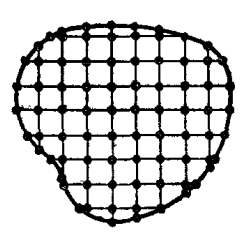
\includegraphics[width=0.5\textwidth]{sector.png}
			\caption{Зависимость количества итераций от шага $\tau$}
		\end{figure}	
		Однако метод теряет порядок по $\tau$, и в итоге получается безусловно устойчивая схема 
		с порядком $O(\tau + \sum_{i} h^2_i)$.
		\item Можно ли использовать метод переменных направлений
		для решения пространственных и вообще n-мерных задач?
		\newline
		{\bfseries Ответ. } 
		Можно использовать следующий метод 
		\begin{gather*}
			\frac{y^{k+1/n} - y^k}{\tau/n} = \Lambda_1 y^{k+1/n} + \Lambda_2 y^k
			+ \ldots + \Lambda_n y^k  + \phi \\
			\frac{y^{k+2/n} - y^{k+1/n}}{\tau/n} = \Lambda_1 y^{k+1/n} + \Lambda_2 y^{k+2/n}
			+ \ldots + \Lambda_n y^{k+1/n}  + \phi \\
			\vdots \\ 
			\frac{y^{k+1} - y^{k+(n-1)/n}}{\tau/n} = \Lambda_1 y^{k+(n-1)/n} + \Lambda_2 y^{k+(n-1)/n}
			+ \ldots + \Lambda_n y^{k+1}  + \phi,
		\end{gather*}
		где $n$ -- размерность пространства.
		В силу несимметричности схемы, компенсация ошибок будет осутствовать, поэтому 
		схема не будет аппроксимировать уравнение. 
		Для такой задачи можно использовать метод дробных шагов.

		Рассмотрим метод дробных шагов подробнее. 
		Будем искать решение на промежуточных слоях с помощью следующей схемы 
		\begin{gather*}
			\frac{1}{\tau}(\hat{w}_\alpha - w_\alpha) = \frac{1}{2} \Lambda_\alpha
			\hat{w}_\alpha (\hat{w}_\alpha + w_\alpha), \quad  \alpha = 1, 2, \ldots, n \\ 
			w_1 = y, w_2 = \hat{w}_1, w_3 = \hat{w}_2, \ldots, w_p = \hat{w}_{p-1},
			\hat{y} = \hat{w}_p
		\end{gather*}
		На целых слоях схема обладает $O(\tau^2 + \sum_{\alpha} h_\alpha^2)$
		\item Можно ли использовать метод переменных направлений
		на неравномерных сетках?
		\newline
		{\bfseries Ответ. } 
		Да.
		\begin{gather*}
			\frac{y^{k+1/2} - y^k}{\tau/2} = \Lambda_1 y^{k+1/2} + \Lambda_2 y^k \\ 
			\frac{y^{k+1} - y^{k+1/2}}{\tau/2} = \Lambda_1 y^{k+1/2} + \Lambda_2 y^{k+1} 
		\end{gather*}
		где $\Lambda_1, \Lambda_2 $
		
		\begin{gather*}
			\Lambda_1y^k = \frac{y^k_{i-1,j} - 2y^k_{i,j} + y^k_{i+1,j}}{(h^1_i)^2} \\
			\Lambda_2y^k = \frac{y^k_{i,j-1} - 2y^k_{i,j} + y^k_{i,j+1}}{(h^2_i)^2} \\
		\end{gather*}
		При выборе шагов таким образом, что 
		выполняется условия устойчивости прогонки, данный метод можно использовать 
		на неравномерных сетках.
		Но стоит отметить, что тогда условие симметрии пропадает, из-за этого перестает 
		взаимноуничтожаться условный порядок сходимости, что в следствии уменьшает итоговый
		порядок до первого по $\tau$.

	\end{enumerate}

	\section{Результаты}
	\begin{figure}[H]
        \centering
        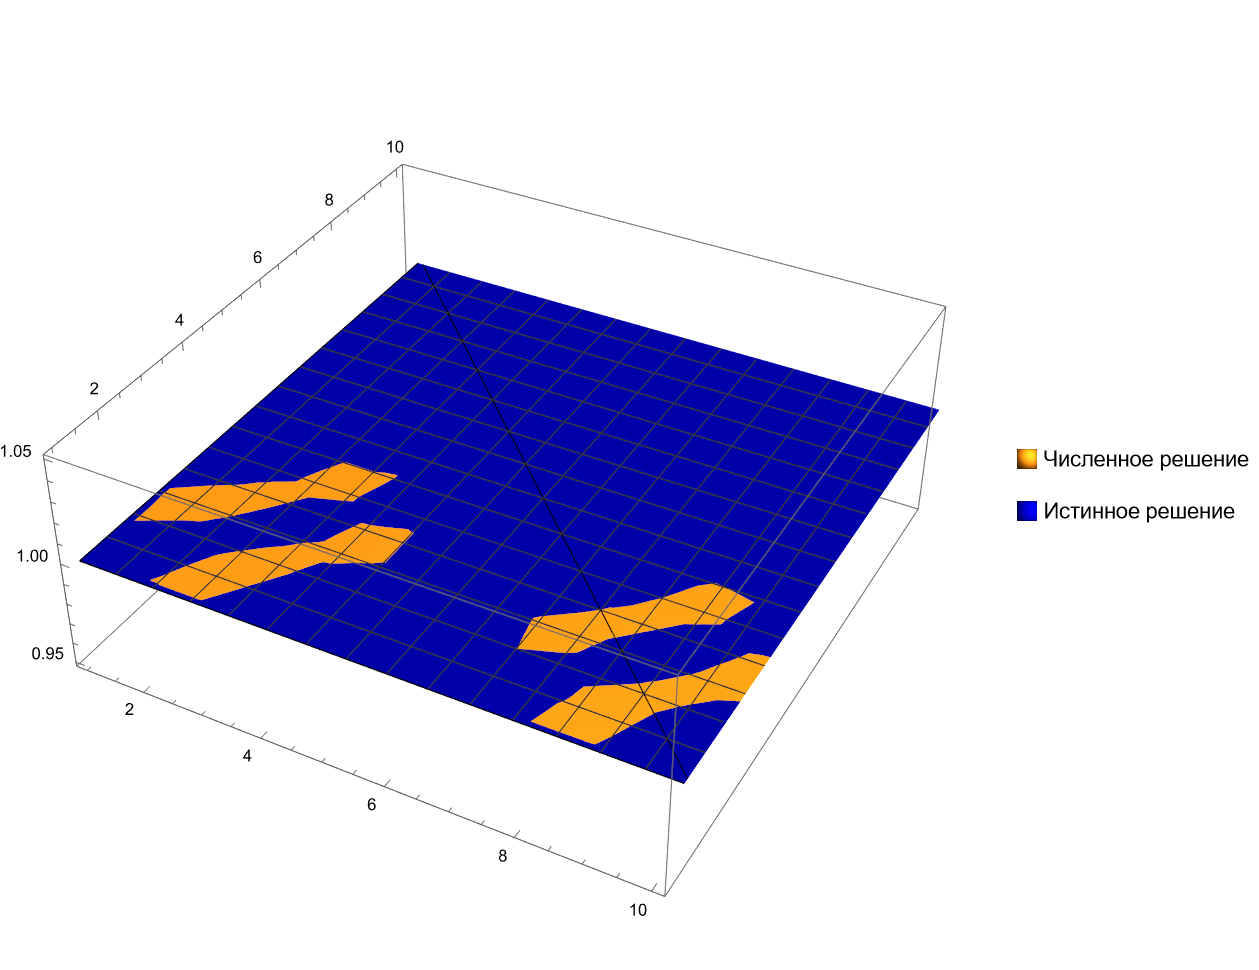
\includegraphics[width=\textwidth]{test1.png}
        \caption{Пример 1. График численного и истинного решений}
    \end{figure}
	\begin{figure}[H]
        \centering
        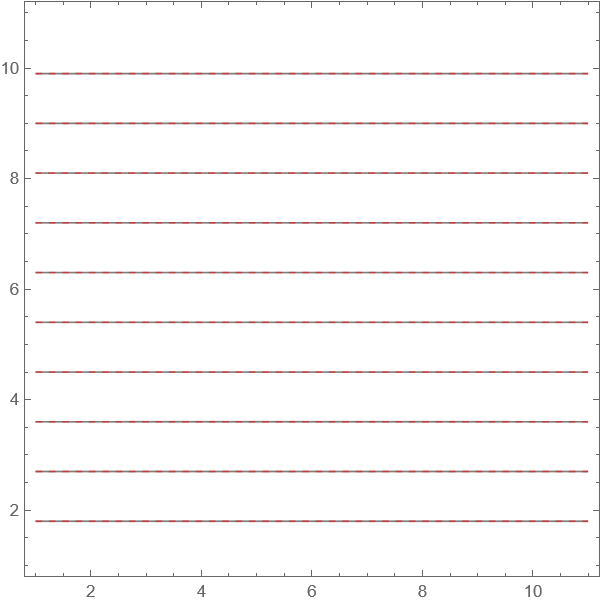
\includegraphics[width=\textwidth]{test2.png}
        \caption{Пример 2. График численного и истинного решений.
		 Красные линии уровня - линии уровня истинного решения, черные линии уровня - 
		 линии уровня численного решения}
    \end{figure}
	\begin{figure}[H]
        \centering
        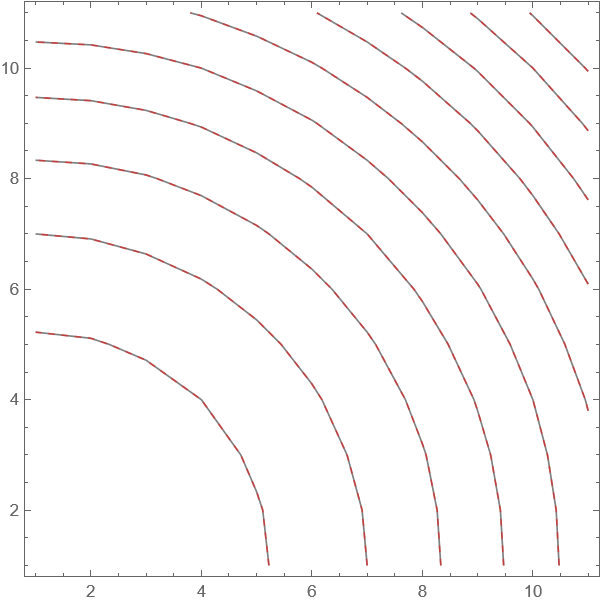
\includegraphics[width=\textwidth]{test3.png}
        \caption{Пример 3. График численного и истинного решений.
		 Красные линии уровня - линии уровня истинного решения, черные линии уровня - 
		 линии уровня численного решения}
    \end{figure}
		\begin{figure}[H]
        \centering
        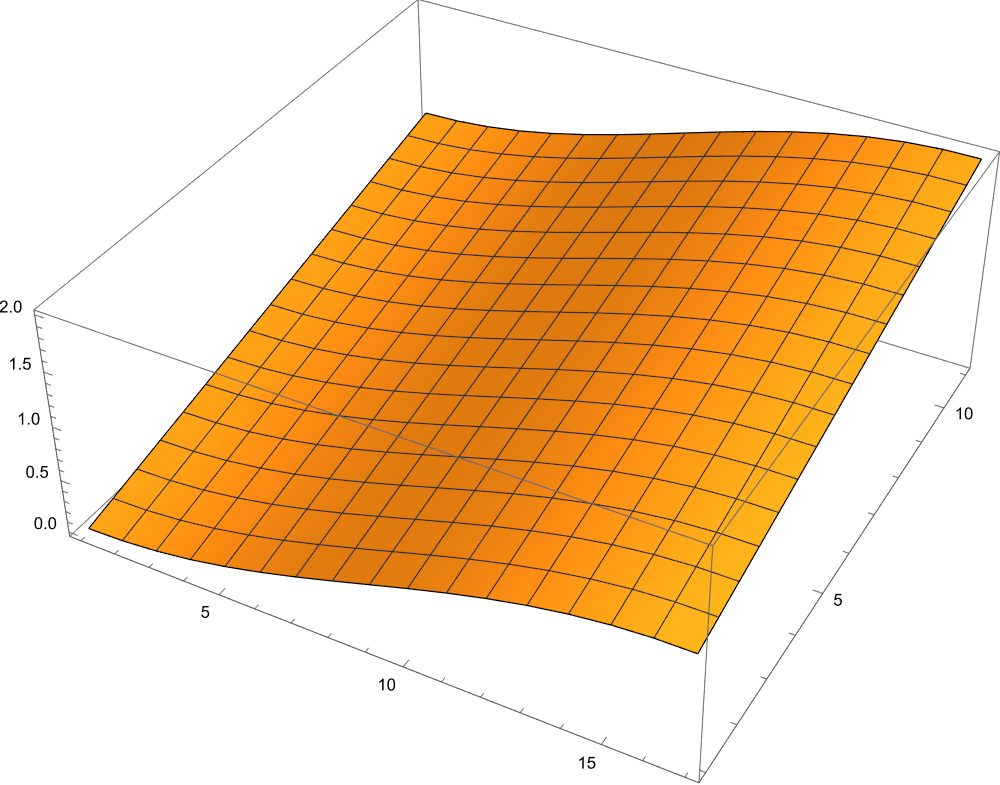
\includegraphics[width=\textwidth]{var1_2.png}
        \caption{Пример для варианта 1. График численного решения}
    \end{figure}

	\section{Порядки}
	Порядки вычислены для следующей задачи
	\begin{gather*}
		u_t - \Delta u = 0, \\ 
		u|_{t=0} = \sin(2 \pi x) \sin(\pi y)\\
		u|_{(x,y) \in \partial D} = 0, \\
		D = [0,1] \times  [0,1].
	\end{gather*}
	Её аналитическое решение определяется 
	\begin{equation*}
		u(x,y, t) = e^{-5\pi^2 t} \sin(2\pi x) \sin(\pi y)
	\end{equation*}
	\begin{table}[H]
		\centering
		\caption{Порядок аппроксимации}
		\begin{tabular}{|c|c|}
			\hline
			Шаг сетки & $z_{n-1} / z_n$ \\ \hline
			$h_1, h_2, \tau$ & --- \\ \hline 
			$q h_1, q h_2, q \tau$ &  3.88543 \\ \hline 
			$q^2 h_1, q^2 h_2,  q^2 \tau$ & 4.0218 \\ \hline 
			$q^3 h_1, q^3 h_2, q^3 \tau$ & 4.00548 \\ \hline 
			$q^4 h_1,q^4 h_2, q^{4} \tau$ & 4.00034 \\ \hline 
	
		\end{tabular}
	\end{table}
	\section{Оптимальные шаги}
	\begin{figure}[H]
        \centering
        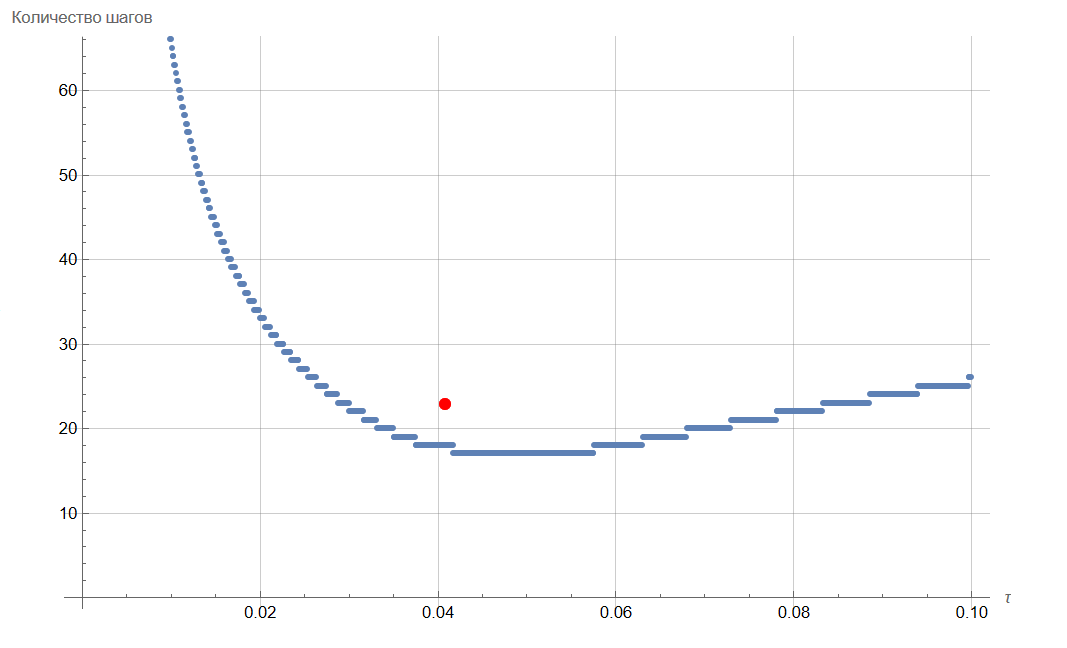
\includegraphics[width=\textwidth]{optimal_step.png}
        \caption{Зависимость количества итераций от шага $\tau$}
    \end{figure}
	При шаге $\tau = 0.041$ (теоретическая оценка) получилась погрешность 
	$\Delta = 1.18087e-06$, при $\tau = 0.05$ (практическая оценка) получилась 
	погрешность $\Delta = 4.14243e-06$.
\end{document}
